% !TeX program = xelatex
% !BIB program = bibtex
% 使用方法：仅替换原项目中的 main.tex，其余文件和目录保持原样。
% 全部摘要、正文、致谢和附录均在本文件内，不拆分为其他 tex 文件。
\documentclass[bachelor]{njupthesis}

% 沿用原文件的目录设置：目录中不显示三级标题。
\makeatletter
\renewcommand{\l@subsection}[2]{}
\makeatother

% ==================== 论文基本信息 ====================
% 以下均为占位信息，请按自己的实际情况填写。
\title{本科毕业设计（论文）题目}
\author{学生姓名}
\advisor{指导教师姓名}
\school{指导单位名称}
\major{专业名称}
\studentclass{} % 班级，可留空
\studentid{00000000}
\graduateyear{2026}
\begindate{20XX年XX月XX日}
\finishdate{20XX年XX月XX日}
\createdate{20XX}{X}{X}

% 继续使用原有 pic 目录。模板默认不插入签名。
% 如需使用已有示例签名，可在自己的论文副本中填写 \authorsign{示例签名}。
\authorsign{示例签名.jpg}
\advisorsign{}

\begin{document}

% 前置页不建立重复页码锚点，不影响原模板的视觉排版。
\hypersetup{pageanchor=false}
\makecover % 封面和原创性声明，样式由原 njupthesis.cls 提供

% ==================== 中文摘要 ====================
\begin{chineseabstract}
此处填写中文摘要。摘要应独立、完整地概述论文的研究目的、研究方法、主要结果和结论，使读者不阅读全文也能够了解论文的核心内容。摘要应与正文一致，避免只介绍研究背景而不交代具体工作。

第一部分简要说明研究背景、需要解决的问题及研究目的。第二部分概述采用的理论、方法、技术路线或实施方案，突出本人完成的主要工作。第三部分给出能够支持结论的主要结果，必要时使用具有代表性的定量指标。

最后总结研究结论、适用条件和实际意义。正式写作时，请将上述说明全部替换为自己论文的摘要，不保留模板提示语，也不把演示数据作为真实研究结果。

\chinesekeyword{关键词一；关键词二；关键词三；关键词四}
\end{chineseabstract}

% ==================== 英文摘要 ====================
\begin{englishabstract}
Replace this text with the English abstract of your thesis. The abstract should provide a concise and self-contained account of the research objective, methods, main results, and conclusions.

First, state the problem and the objective of the study. Then describe the methods and the work carried out. Report the main findings with appropriate quantitative evidence when available. Finally, summarize the conclusions, their scope, and their practical significance.

The English abstract should correspond to the Chinese abstract in both content and terminology. The text in this template is an instruction for writing and does not describe an actual research study.

\englishkeyword{Keyword one; Keyword two; Keyword three; Keyword four}
\end{englishabstract}

\thesistableofcontents % 目录
\thesischapterexordium % 正文开始，沿用原模板页眉和页码设置
\hypersetup{pageanchor=true}

% ==================== 第一章 ====================
\chapter{绪论}
\label{chap:introduction}

\section{研究背景及意义}
此处介绍课题所处的研究背景、实际需求和需要解决的问题。背景应与论文的具体目标直接相关，可从应用场景、已有技术的不足以及研究问题的价值等方面展开。

研究意义应说明完成本课题能够带来什么具体帮助，例如改善某项性能、解释某种现象或提供一种可复核的方法。正式写作时，应以实际资料支持判断，避免只使用宽泛的评价性表述。

\section{国内外研究现状}
此处围绕论文的核心问题整理已有研究。可以按方法类型、关键技术或发展阶段组织内容，说明已有工作的思路、适用条件及不足，并据此引出本文的研究目标。

下面仅演示文献引用的写法，继续调用原项目 \texttt{reference.bib} 中已有的条目：单篇引用示例\cite{tang2015}，多篇引用示例\cite{wang2016,chen2019}。这些引用只用于展示编号和参考文献列表的效果，不用于支持本模板中的通用写作说明。写作时请改为实际使用的文献。

\section{研究内容与论文结构}
此处明确论文要完成的研究任务，并说明各章之间的联系。本模板用以下内容演示论文的组织方式：
\begin{enumerate}
  \item 说明研究问题、基本概念和评价指标。
  \item 介绍研究方法、实施步骤及关键设计。
  \item 给出结果、分析依据和方法的适用范围。
  \item 总结主要工作，并说明不足与后续研究方向。
\end{enumerate}

本文的理论与方法见\ref{chap:methods}，方案说明见\ref{chap:design}，结果分析见\ref{chap:results}，总结与展望见\ref{chap:conclusion}。这些章节名称可按课题实际需要修改。

% ==================== 第二章 ====================
\chapter{相关理论与研究方法}
\label{chap:methods}

\section{基本概念与符号说明}
此处说明研究所需的基本概念、理论依据和适用条件。对于后文反复出现的符号，应在首次出现时给出定义，并在全文保持含义和单位一致。

正文使用空行分隔自然段，不必在每段末尾添加强制换行。三级标题的写法见下文，目录的显示层级继续沿用原文件设置。

\subsection{三级标题示例}
此处填写本小节内容。同一层级的标题应采用一致的表达方式。标题不宜过长，也不宜用过深的层级代替必要的段落组织。

\section{数学公式与交叉引用}
短公式可以放在正文中，例如样本数量记为 $n$。需要编号的公式可以使用公式环境。设观测值为 $x_1,x_2,\ldots,x_n$，样本均值为
\begin{equation}
  \bar{x}=\frac{1}{n}\sum_{i=1}^{n}x_i,
  \label{eq:mean}
\end{equation}
其中，$x_i$ 表示第 $i$ 个观测值，$n$ 表示观测值数量。

当 $n\geq2$ 时，样本标准差可写为
\begin{equation}
  s=\sqrt{\frac{1}{n-1}\sum_{i=1}^{n}(x_i-\bar{x})^2}.
  \label{eq:std}
\end{equation}
在正文中可使用式~\eqref{eq:mean}~和式~\eqref{eq:std}~进行交叉引用。请让公式编号自动生成，不要手动输入编号。

\section{方法与评价指标}
此处说明采用该方法的原因、实现步骤和评价依据。如果方法依赖某些前提，应明确列出其适用条件；如果需要比较不同方案，应统一评价指标和数据处理方式。

必要的补充解释可以使用脚注。\footnote{此处为脚注示例，可用于解释术语或提供简短补充信息。}
脚注不应代替正文中的关键分析，引用文献仍应使用文献引用命令。

\section{本章小结}
此处概括本章介绍的理论与方法，并说明它们如何支持后续方案设计。小结应围绕本章实际内容展开，不引入正文中尚未说明的新结论。

% ==================== 第三章 ====================
\chapter{方案设计与实现}
\label{chap:design}

\section{总体方案}
此处介绍研究方案的目标、组成和实施顺序。可以结合实际课题说明输入条件、处理过程、关键参数和预期输出，突出各部分之间的联系。

图~\ref{fig:example}~演示单幅图片的排版。这里使用占位框，因此不需要增加、移动或重命名原项目中的任何图片文件。

\begin{figure}[htbp]
  \centering
  \fbox{\parbox[c][3.5cm][c]{0.75\textwidth}{\centering
    图片占位区域\\[6pt]
    请替换为自己的研究图片}}
  % 使用原 pic 目录图片时，可将上面的占位框替换为：
  % 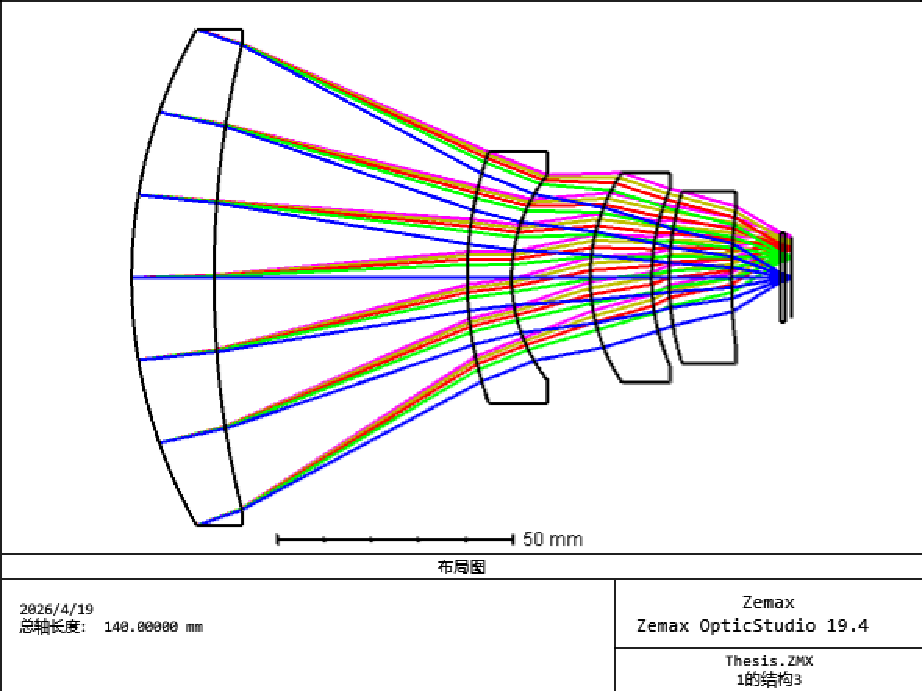
\includegraphics[width=0.8\textwidth]{pic/2D图.pdf}
  \caption{单幅图片的排版示例}
  \label{fig:example}
\end{figure}

插图应先在正文中被提及，再放置在适当位置。图题应说明图片内容，图中的文字、图例和标注在缩放后也应清晰可读。

\section{关键参数与表格示例}
表~\ref{tab:parameters}~展示三线表的基本写法。以下数值均为排版演示，不代表真实系统参数。正式写作时，请替换为研究中使用的参数、单位及其来源。

\begin{table}[htbp]
  \centering
  \caption{参数表格示例（仅用于排版演示）}
  \label{tab:parameters}
  \begin{tabularx}{0.9\textwidth}{lYY}
    \toprule
    参数名称 & 符号 & 演示值 \\
    \midrule
    样本数量 & $n$ & 5 \\
    长度参数 & $L/\mathrm{mm}$ & 20 \\
    时间参数 & $t/\mathrm{s}$ & 10 \\
    \bottomrule
  \end{tabularx}
\end{table}

\section{并列子图示例}
图~\ref{fig:comparison}~演示原模板已有的子图功能，继续使用原类文件加载的 \texttt{subfigure}，无需更换宏包或修改图片目录。

\begin{figure}[htbp]
  \centering
  \subfigure[情形一]{%
    \fbox{\parbox[c][3cm][c]{0.38\textwidth}{\centering 子图占位区域一}}}
  \hfill
  \subfigure[情形二]{%
    \fbox{\parbox[c][3cm][c]{0.38\textwidth}{\centering 子图占位区域二}}}
  \caption{并列子图的排版示例}
  \label{fig:comparison}
\end{figure}

\section{本章小结}
此处总结方案设计与实现过程中的关键内容。对方案效果的判断，应在后续结果分析中结合实际数据给出依据。

% ==================== 第四章 ====================
\chapter{结果分析与讨论}
\label{chap:results}

\section{数据来源与处理方法}
此处说明数据的获取方式、实验或计算条件以及处理流程。若数据来自公开资料，应给出来源；若来自实验，应交代采集条件、样本数量和异常数据的处理方法。

本章使用两组人工构造的数值演示表格与结果分析，不对应真实实验。条件一为 $8,9,10,11,12$，条件二为 $9,10,10,10,11$，均为无量纲数据。

\section{结果展示}
根据式~\eqref{eq:mean}~和式~\eqref{eq:std}~计算得到表~\ref{tab:results}~中的结果。两组数据的均值均为 $10$，样本标准差分别约为 $1.581$ 和 $0.707$。

\begin{table}[htbp]
  \centering
  \caption{人工演示数据的统计结果}
  \label{tab:results}
  \begin{tabular}{lccc}
    \toprule
    条件 & 样本数量 & 均值 & 样本标准差 \\
    \midrule
    条件一 & 5 & 10.000 & 1.581 \\
    条件二 & 5 & 10.000 & 0.707 \\
    \bottomrule
  \end{tabular}
\end{table}

\section{结果讨论与适用范围}
两组演示数据的均值相同，条件二的数值更加集中。这一结果只说明本例中数值的离散程度，不能据此推断真实研究中某种方法一定更优。

正式论文中的讨论应结合研究目标解释结果，区分能够直接观察到的事实与进一步提出的解释，并说明样本量、实验条件和评价方法带来的限制。

\section{本章小结}
此处总结本章得到的主要结果及其依据。请使用能够从数据中得到支持的结论，不把排版示例或尚未验证的推测写成研究成果。

% ==================== 第五章 ====================
\chapter{总结与展望}
\label{chap:conclusion}

\section{研究总结}
此处围绕论文的研究目标，概括已经完成的主要工作、采用的方法和得到的结果。总结应与前文的研究任务相对应，不简单重复摘要，也不加入正文中没有讨论的新结论。

可以按以下顺序组织：首先说明解决了什么问题；其次概括完成了哪些具体工作；最后给出主要结果及其适用条件。创新点应以实际工作为基础，准确说明与已有方法的差别。

\section{不足与展望}
此处说明研究中仍然存在的不足，例如数据范围有限、验证条件不充分或方法仍有改进空间。后续工作应具体、可执行，并与本文已经识别的问题直接相关。

% ==================== 结束语 ====================
% 如不需要结束语，可删除下面命令及其后的对应段落。
\thesisconclusion
此处填写结束语，可简要回顾毕业设计的工作过程、学习收获和实践体会。有关研究成果的总结应以正文为依据，避免重复堆叠相同结论。

% ==================== 致谢 ====================
\thesisacknowledgement
此处填写致谢，感谢在课题研究、实验实施和论文写作中提供实际帮助的指导教师、同学及其他人员。致谢内容应真实、得体，正式使用时请替换为自己的表达。

本模板沿用原项目的排版样式。原项目中说明的模板来源包括 \url{https://github.com/musnows/NJUPT-Bachelor} 及其上游贡献者；此处保留来源说明。

% ==================== 参考文献 ====================
% 继续由原类文件读取原 reference.bib，不另建文献文件。
% 本地分组使参考文献字号不影响后面的附录正文。
\begingroup
\thesisreference
\endgroup

% ==================== 附录 ====================
% 如不需要附录，可删除从 \thesisappendix 到 \end{document} 前的内容。
% 继续使用原 njupthesis.cls 提供的附录命令。
\thesisappendix
以下为程序排版示例，代码与前文两组人工数据对应。正式论文可在此放置补充推导、程序片段或其他支持材料。

\begin{lstlisting}[language=Python,caption={演示数据统计程序}]
from statistics import mean, stdev

samples = {
    "condition_1": [8, 9, 10, 11, 12],
    "condition_2": [9, 10, 10, 10, 11],
}

for name, values in samples.items():
    print(name, round(mean(values), 3), round(stdev(values), 3))
\end{lstlisting}

\end{document}
